%=================================================================
\chapter{Systematic Literature Mapping}
\label{chap:slm}
%=================================================================

% http://200.132.136.13/Thoth/

% Esse capítulo descreve os procedimentos adotados para a investigação da literatura realizada para este estudo. 
% Para este propósito ser alcançado foi realizado o planejamento e a execução de um Mapeamento da Literatura. 
% Para isto foram aplicadas diretrizes bem estabelecidas conceitualmente com base em propostas de diversos trabalhos~\cite{Kitchenham:2007, Petersen:2008, Nakagawa:2017}.  
This chapter describes the procedures adopted for the investigation of the literature carried out for this study.
For achieving this purpose, we have carried out the planning and execution of a Systematic Literature Mapping.
For this, we have applied conceptually well-established guidelines based on proposals from several works~\cite{Kitchenham:2007, Petersen:2008, Nakagawa:2017}.

% Transformation Mechanisms of Relational Database Models: A Systematic Mapping

% Description
% Mapping of transformation heuristics/strategies/guidelines for generation of relational databases

% Objectives
% Gather similar studies evaluating them critically in their methodology and bringing them together in a careful analysis.

%------------------------------------------------------------------------------
\section{Protocol}\label{sec:slr_protocol}
%------------------------------------------------------------------------------

% Um Mapeamento Sistemático de Literatura é útil para pesquisadores e profissionais pois fornecem visões abrangentes sobre o estado da arte em uma área específica.
% Neste estudo conduziu-se um mapeamento utilizando o processo de definido por Petersen~\cite{Petersen:2008}.

A Systematic Literature Mapping is helpful for researchers and practitioners as it provides comprehensive insights into the state-of-the-art in a specific area.
In this study, we have conducted a mapping using the process defined by Petersen~\cite{Petersen:2008}.

%#################################################################
\subsection{Research Questions} \label{ssec_slm:researchQuestions}
%#################################################################

% Levando-se em consideração o objetivo geral deste trabalho, o qual é desenvolver desenvolver uma ferramenta de modelagem para a modelagem conceitual de BDs que implemente uma DSL previamente proposta, foram formulados os seguintes questionamentos com o objetivo de investigar os mecanismos de transformação utilizados por DSLs:
Taking into account the general objective of this work, which is to develop a modeling tool for the conceptual modeling of \acp{db} that implements a previously proposed DSL, we have formulated the following research questions to investigate the transformation mechanisms used by \acp{dsl}:

\begin{itemize}
    \item \textbf{RQ1.} What is the state of the art of mechanisms for transforming conceptual models?
    % \item \textbf{RQ2.} What transformation mechanisms among conceptual models are applied in the context of DSLs?
    \item \textbf{RQ2.} What are transformation mechanisms applied among conceptual models in the context of DSLs?
    \item \textbf{RQ3.} What representations of database resources do the transformation mechanisms support?
\end{itemize}

%#################################################################
\subsection{Research Sources} \label{ssec_slm:researchSources}
%#################################################################

% As bibliotecas digitais são a principal fonte de busca em um \ac{SLM}~\cite{Petersen:2008}. 
% Para a escolha das fontes de busca desse \ac{SLM} são considerados três requisitos obrigatórios que as bases devem contemplar: 
% \textbf{(i)} possuir mecanismo de pesquisa baseado na \textit{Web}; 
% \textbf{(ii)} ser capaz de usar palavras-chave durante a pesquisa, e;
% \textbf{(iii)} abranger estudos primários da grande área da Ciência da Computação.
% Na Tabela \ref{tab:BasesDePesquisa} são listadas as bibliotecas digitais selecionadas para este mapeamento.
Digital libraries are the principal source of research in an systematic literature mapping~\cite{Petersen:2008}.
To choose the research sources for this systematic literature mapping, we have considered three mandatory requirements that the databases must meet:
\textbf{(i)} have search engine based on \textit{Web};
\textbf{(ii)} be able to use keywords when searching, and;
\textbf{(iii)} cover primary studies Computer Science area.
Table \ref{tab:reserchSources} lists the digital libraries selected for this mapping.
        
\rowcolors{1}{gray!15}{white}
\begin{table}[!ht]
    \centering
    \scriptsize
    \caption{Digital libraries used.}
    \label{tab:reserchSources}
    \begin{tabular}{m{4cm}m{4cm}m{4cm}}
    \bottomrule
    \rowcolor[HTML]{C0C0C0}
    \textbf{Source} & \textbf{Address} & \textbf{Type} \\ 
    \hline
    ACM Digital library & \textit{dl.acm.org}           & Hybrid\\
    IEEE Xplore         & \textit{ieeexplore.ieee.org}  & Bibliographic Database \\ 
    Scopus       & \textit{scopus.com}   & Search Engine \\
    Google Scholar        & \textit{scholar.google.com}    & Search Engine \\ 
    \toprule
    \end{tabular}
    \fonte{Adapted from~\cite{Nakagawa:2017}.}
\end{table}

%#################################################################
\subsection{Search String} \label{ssec_slm:searchString}
%#################################################################

% A elaboração da \textit{string} de busca não é uma tarefa trivial. 
% A identificação de uma combinação de termos que permitam encontrar o maior número de estudos primários relevantes de forma objetiva necessita, na maioria dos casos, de experiência e profundo conhecimento sobre a área de pesquisa abordada.  
The elaboration of the search string is not a trivial task.
The identification of a terms combination that allow finding the greatest number of relevant primary studies in an objective way requires, in most cases, experience and in-depth knowledge of the research area addressed.

% Para a formação da string de busca é fundamental definir um conjunto de palavras referentes ao tema de pesquisa, bem como os sinônimos considerados expressivos. 
% Estes termos devem representar de forma abrangente o tema central do estudo. 
% Para este trabalho foram estabelecidos os termos e sinônimos cuja sua combinação gerou a string genérica da Firgura \ref{fig:searchString}. 
% Posteriormente, as strings foram derivadas para se adequarem as restrições de cada mecanismo de busca, sendo apresentadas na Tabela \ref{tab:StringsDatabases}.
For the search string definition, it is essential to define a set of words referring to the research topic as well as the synonyms are considered expressive. 
These terms should comprehensively represent the central theme of the study. 
For this work, we have established the terms and synonyms whose combination generated the generic string shown in Figure \ref{fig:searchString}. 
Subsequently, Table \ref{tab:StringsDatabases} presents the strings that we have derived for fitting the constraints of each search engine. 

\begin{figure}[htb]
\centering
\caption{Generic search string.}
\label{fig:searchString}
\fbox{\
\small
\parbox{14cm}{
\centering
\tiny\texttt{
("Domain-Specific Language" OR "Domain Specific Language" OR DSL OR \linebreak "Domain-Specific Modeling Language" OR "Domain Specific Modeling Language" \linebreak OR DSML OR "Domain-Specific Modeling" OR DSM) \linebreak 
AND \linebreak
(Entity-Relationship OR ER OR "Enhanced Entity-Relationship" OR \linebreak EER OR "Entity Relationship Diagram" OR ERD) \linebreak 
AND \linebreak
("Model Transformation" OR Model-to-Text OR M2T OR Model-to-Model OR \linebreak M2M OR "Code Generation")}}}
\fonte{Author.}
\end{figure}


\begin{table}[!htb]
\caption{Search strings derived by sources.}
\label{tab:StringsDatabases}
\tiny
\begin{tabular}{m{1.0cm}m{14.0cm}}
\bottomrule
\textbf{Source} & \textbf{Search String} \\
\hline
\T ACM & \texttt{Abstract:(("Domain-Specific Language" OR "Domain Specific Language" OR DSL OR "Domain-Specific Modeling Language" OR "Domain Specific Modeling Language" OR DSML OR "Domain-Specific Modeling" OR DSM) \linebreak AND \linebreak (Entity-Relationship OR ER OR "Enhanced Entity-Relationship" OR EER OR "Entity Relationship Diagram" OR ERD) \linebreak AND \linebreak ("Model Transformation" OR Model-to-Text OR M2T OR Model-to-Model OR M2M OR "Code Generation")} \\
\midrule
\T Google & \texttt{("Domain-Specific Language" OR "Domain-Specific Modeling Language" OR "Domain-Specific Modeling") \linebreak AND \linebreak (Entity-Relationship OR "Enhanced Entity-Relationship") \linebreak AND \linebreak ("Model Transformation" OR Model-to-Text OR M2T OR Model-to-Model OR M2M OR "Code Generation")} \\
\midrule
\T Scopus & \texttt{TITLE-ABS-KEY ( "Domain-Specific Language"  OR  "Domain Specific Language"  OR  dsl  OR  "Domain-Specific Modeling Language"  OR  "Domain Specific Modeling Language"  OR  dsm  OR  "Domain-Specific Modeling"  OR  dsm )  \linebreak AND \linebreak ( entity-relationship  OR  per  OR  "Enhanced Entity-Relationship"  OR  eer  OR  "Entity Relationship Diagram"  OR  erd ) \linebreak AND \linebreak ( "Model Transformation"  OR  model-to-text  OR  met  OR  model-to-model  OR  mcm  OR  "code generation")} \\
\midrule
\T IEEE & \texttt{(("Full Text .AND. Metadata":"Domain-Specific Language" OR "Full Text .AND. Metadata":"Domain Specific Language" OR "Full Text .AND. Metadata":DSL OR "Full Text .AND. Metadata":"Domain-Specific Modeling Language" OR "Full Text .AND. Metadata":"Domain Specific Modeling Language" OR "Full Text .AND. Metadata":DSML OR "Full Text .AND. Metadata":"Domain-Specific Modeling" OR "Full Text .AND. Metadata"::DSM) \linebreak AND \linebreak ("Full Text .AND. Metadata":"Entity-Relationship" OR "Full Text .AND. Metadata"::ER OR "Full Text .AND. Metadata"::"Enhanced Entity-Relationship" OR "Full Text .AND. Metadata"::EER OR "Full Text .AND. Metadata":"Entity Relationship Diagram" OR "Full Text .AND. Metadata":ERD) \linebreak AND \linebreak ("Full Text .AND. Metadata":"Model Transformation" OR "Full Text .AND. Metadata":"Model-to-Text" OR "Full Text .AND. Metadata":M2T OR "Full Text .AND. Metadata":"Model-to-Model" OR "Full Text .AND. Metadata":M2M OR "Full Text .AND. Metadata":"Code Generation")} \\
\noalign{\smallskip} 
\toprule
\end{tabular}
\end{table}    

% Para a geração das strings, bem como todo o processo de mapeamento, foi utilizado o apoio da ferramenta Thoth\footnote{Thoth Tool: \url{http://lesse.com.br/tools/thoth/}}, uma ferramenta web que fornece apoiar processos de revisão sistemáticas~\cite{thoth:2019}. 
% A string para a ACM era a versão base gerada pela ferramenta, limitando ao conjunto \textit{The ACM Full-Text Collection} (com 606,408 registros na época) e limitando ao abstract.
For the generation of strings as far as the entire mapping process, we have used the support of the Thoth\footnote{Thoth Tool: \url{http://lesse.com.br/tools/thoth/}} tool, a web tool that provides support for systematic review processes~\cite{thoth:2019}.
The string for the ACM was the base version generated by the tool, limiting it to \textit{The ACM Full-Text Collection} set (with 606,408 records at the time) and limiting it to the abstract.
% No Google Scholar a string foi limitada a 256 caracteres, sendo que os hífens não fazem diferença. 
% A string derivada que foi usada ficou com exatos 256 caracteres e os resultados trouxeram estudos aparentemente relevantes.
In Google Scholar the string was limited to 256 characters, with hyphens making no difference.
The derived string that was used was exactly 256 characters long and the results brought relevant studies.
% A string para a IEEE precisou ser limitado a 20 termos.
% O resultado foi obtido buscando full text e metadata dos estudos. 
% Isso foi necessário por quando feita apenas verificando os abstracts havia o retorno de 0 resultados.
The string for IEEE needed to be limited to 20 terms.
The result was obtained by searching full text and metadata of the studies.
This was necessary because when only checking the abstracts, no results were returned.

%#################################################################
\subsection{Selection Criteria} \label{ssec_slm:selectionCriteria}
%#################################################################

% Segundo~\cite{Kitchenham:2007}, os critérios de inclusão indicam por qual ou quais parâmetros um estudo é incluído, ou seja, considerado relevante. 
% Da mesma forma, os critérios de exclusão indicam por qual ou quais parâmetros um estudo é excluído, ou seja, considerado não relevante na pesquisa realizada. 
% Para o este trabalho foram determinados os critérios de seleção listados a seguir.
According to~\cite{Kitchenham:2007}, the inclusion criteria indicate by which parameters a study is included, that is, considered relevant.
Likewise, the exclusion criteria indicate by which parameters a study is excluded, that is, considered not relevant in the research.
For this work, we have determined the selection criteria listed below.

\begin{itemize}
    \item \textbf{Inclusion Criteria (IC)}    
    \begin{itemize}
        \item \textbf{IC1.} Primary study reporting mechanisms, guidelines, heuristics or strategies for transforming conceptual data models of relational databases. 
    \end{itemize}
    \item \textbf{Exclusion Criteria (EC)}
    \begin{itemize}
        \item \textbf{EC1.} Duplicate primary studies;
        \item \textbf{EC2.} Primary studies with less than 4 pages;
        \item \textbf{EC3.} Primary study that is not written in English;
        \item \textbf{EC4.} Secondary and tertiary studies;
        \item \textbf{EC5.} Primary study that does not provide full access;
        \item \textbf{EC6.} Primary study does not satisfy the inclusion criteria.
    \end{itemize}
\end{itemize}

 
 %#################################################################
\subsection{Quality Assessment Criteria} \label{ssec_slm:qualityCriteria}
%#################################################################

% Segundo~\cite{Nakagawa:2017}, embora exemplos de formulários de avaliação de qualidade possam ser encontrados com certa facilidade na literatura, para a elaboração de critérios e definição de seus pesos os pesquisadores envolvidos em cada revisão ou mapeamento devem levar em consideração as particularidades conforme o tema e as questões de pesquisa.
% Portanto, em pesquisas desse tipo existe total liberdade para definição o número de critérios de qualidade e seus pesos relacionados. 
According to~\cite{Nakagawa:2017}, although we can find with some ease in the literature examples of quality assessment forms for the criteria elaboration and their weights definition, the researchers involved in each review or mapping must consider the particularities depending on the theme and the research questions.
% According to~\cite{Nakagawa:2017}, although examples of quality assessment forms can be found with some ease in the literature, for the elaboration of criteria and definition of their weights, the researchers involved in each review or mapping must take into account the particularities depending on the theme and the research questions.
Therefore, there is complete freedom to define the number of quality assessment criteria and their related weights in this research type.

% Foram definidos três (3) critérios de qualidade para a avaliação dos estudos primários aprovados após a aplicação dos critérios de seleção. 
% Os critérios de qualidade visam quantificar a relevância para que seja possível realizar uma comparação entre os estudos selecionados. 
% Foi definido também uma pontuação para ser atribuída a partir dos critérios de qualidade. 
% Para a definição das pontuações foram estabelecidas siglas para as representar.
We have defined three (3) quality assessment criteria to rate primary studies approved after applying the selection criteria.
The quality assessment criteria aim to quantify the relevance so that it is possible to realize a comparison among the selected studies.
A score was also defined to be assigned based on the quality criteria.
We have established acronyms to define the scores to represent them.

\begin{itemize}
    \item \textbf{G: Good}, the study fully meets the quality assessment criteria;
    \item \textbf{A: Average}, the study partially meets the quality assessment criteria;
    \item \textbf{P: Poor}, the study does not meet the quality assessment criteria.
\end{itemize}

% Para todos os critérios a sigla \textbf{P} (Poor) representava zero (0) e a sigla \textbf{G} (Good) representava o conceito máximo de valor um (1).
% A sigla \textbf{A} (Average) se referia a um meio termo, valendo uma pontuação de 0.5. 
For all criteria, the acronym \textbf{P} (Poor) represents zero (0) and the acronym \textbf{G} (Good) depicts the maximum concept of value one (1).
The acronym \textbf{A} (Average) refers to a middle ground, with a score of 0.5.
% A pontuação máxima possível era, avaliados todos os critérios, três (3.0) e a mínima zero (0). 
% Os critérios de qualidade são apresentados na Tabela \ref{tab:CAQ}.
By the way, the maximum possible score when we evaluated all criteria is three (3.0), and the minimum is zero (0).
Table \ref{tab:QAC} shows the quality assessment criteria.

\rowcolors{1}{gray!15}{white}
\begin{table}[!htb]
    \centering
    %\small
    \footnotesize
    \caption{Quality assessment criteria.}
    \label{tab:QAC}
    \begin{tabular}{l|p{12cm}|c}
    \bottomrule
    \rowcolor[HTML]{C0C0C0}
    \textbf{ID} & \textbf{Description} & \textbf{Weight} 
    \\ 
    \hline
    QC1. & Does the study present refinement techniques, guidelines, mechanisms, or heuristics based on conceptual data models for relational databases? & 1,0 
    \\
    QC2. & Does the study provide details of the model transformation mechanisms? & 1,0 
    \\
    QC3. & Does the study present some evaluation way of the transformation mechanisms presented? & 1,0 
    \\
    \toprule
    \end{tabular}
    \fonte{Author.}
\end{table}

%#################################################################
\subsection{Data Extraction Strategy} \label{ssec_slm:dataExtraction}
%#################################################################

% Definiu-se um formulário de dados para a extração e análise dos dados relevantes contidos nos estudos primários selecionados. 
% A descrição detalhada deste formulário de extração é apresentado na Tabela \ref{tab:DataExtractionForm}.
We have defined a data form for the extraction and analysis of relevant data of the selected primary studies.
Table \ref{tab:DataExtractionForm} presents the detailed description of this extraction form.

\rowcolors{1}{gray!15}{white}
\begin{table}[!htb]
    \centering
    \scriptsize
    \caption{Data extraction form.}
    \label{tab:DataExtractionForm}
    \begin{tabular}{p{5cm}|p{10cm}}
    \bottomrule
    \rowcolor[HTML]{C0C0C0} 
    \textbf{Data} & \textbf{Description} \\
    \hline
    Solution Origin & Organization or University of the study authors
    \\
    Year of Publication & Year of publication of the study
    \\
    Solution Objective & Proposed Solution Description
    \\
    Purpose of the paper & Description of the article's objectives
    \\
    Reported strengths & Description of reported strengths
    \\
    Reported shortcomings & Description of reported shortcomings
    \\
    Database resources & Description of objects supported in the transformation process
    \\
    DSL names & DSLs that apply transformation mechanisms among conceptual data models
    \\
    Transformation mechanism type & Reported Guideline, Heuristic, Strategy or Technique
    \\
    \toprule
    \end{tabular}
    \fonte{Author.}
\end{table}

%#################################################################
\subsection{Selection Process} \label{ssec_slm:selectionProcess}
%#################################################################

% Todas as etapas de seleção também foram realizadas com a ajuda da ferramenta Thoth e um resumo geral é exibido na Figura \ ref {fig: selectionSteps}.
% Inicialmente identificamos um total de 1602 estudos extraídos das quatro (4) fontes consultadas. 
% A etapa seguinte compreendeu a verificação e exclusão de estudos duplicados.
% Isso resultou na exclusão de 139 estudos, restando assim 1463 estudos para a aplicação dos critérios de inclusão e exclusão.
% Nesse ponto os critérios foram aplicados específicamente com base nos títulos, palavras-chave e resumos.
% Após esta tarefa ser terminada, restaram 30 estudos.
We also have performed all selection steps with the help of the Thoth tool, and Figure \ref{fig:selectionSteps} depicts an overview.
Initially, we identified a total of 1602 studies extracted from the four (4) sources consulted.
The next step involved the verification and exclusion of duplicate studies.
This step resulted in the exclusion of 139 studies, leaving 1463 studies to apply the inclusion and exclusion criteria step.
At this point, we have specifically applied the criteria based on titles, keywords, and abstracts.
After this task, we completed the selection process, where 30 studies remained.

\begin{figure}[!htb]
    \centering
    \caption{Selection process steps.}
    \label{fig:selectionSteps}
    

\tikzset{every picture/.style={line width=0.75pt}} %set default line width to 0.75pt        

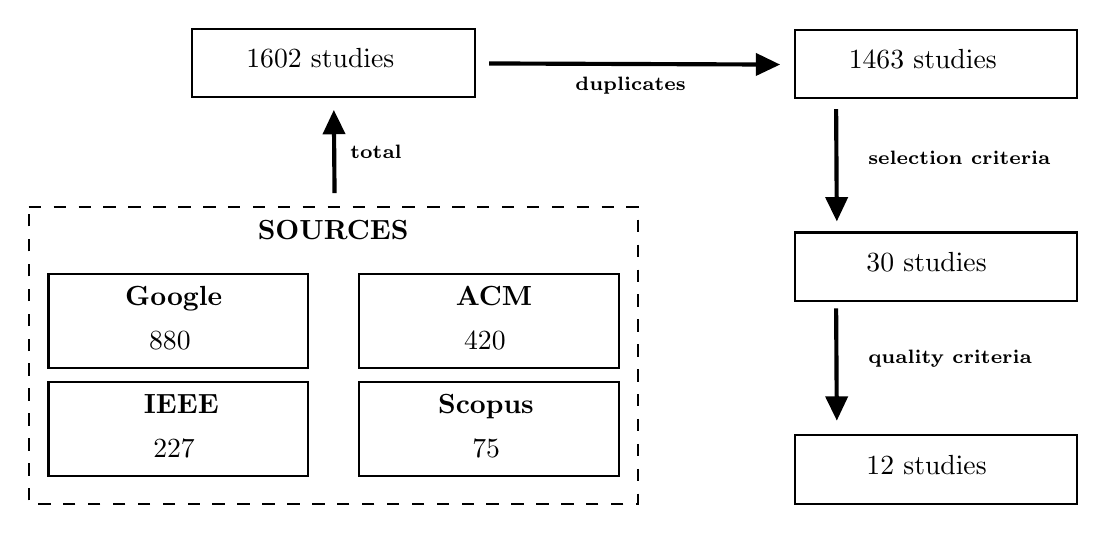
\begin{tikzpicture}[x=0.75pt,y=0.75pt,yscale=-1,xscale=1]
%uncomment if require: \path (0,300); %set diagram left start at 0, and has height of 300

%Shape: Rectangle [id:dp6546352297933162] 
\draw   (17.04,127.79) -- (141.98,127.79) -- (141.98,173.01) -- (17.04,173.01) -- cycle ;

%Shape: Rectangle [id:dp8303551301255043] 
\draw   (166.79,127.79) -- (291.72,127.79) -- (291.72,173.01) -- (166.79,173.01) -- cycle ;

%Shape: Rectangle [id:dp8113957066476918] 
\draw   (17.04,179.76) -- (141.98,179.76) -- (141.98,224.98) -- (17.04,224.98) -- cycle ;

%Shape: Rectangle [id:dp25742759249794456] 
\draw   (166.79,179.76) -- (291.72,179.76) -- (291.72,224.98) -- (166.79,224.98) -- cycle ;


%Shape: Rectangle [id:dp887698650238713] 
\draw  [dash pattern={on 4.5pt off 4.5pt}] (7.5,95.27) -- (301.26,95.27) -- (301.26,238.27) -- (7.5,238.27) -- cycle ;


%Shape: Rectangle [id:dp2249952504303483] 
\draw   (86.25,9.5) -- (222.51,9.5) -- (222.51,42.35) -- (86.25,42.35) -- cycle ;

%Shape: Rectangle [id:dp5429657438012057] 
\draw   (376.5,10) -- (512.76,10) -- (512.76,42.85) -- (376.5,42.85) -- cycle ;

%Shape: Rectangle [id:dp8170922890561967] 
\draw   (376.5,107.7) -- (512.76,107.7) -- (512.76,140.56) -- (376.5,140.56) -- cycle ;

%Shape: Rectangle [id:dp9256107502869182] 
\draw   (376.5,205.42) -- (512.76,205.42) -- (512.76,238.27) -- (376.5,238.27) -- cycle ;

%Straight Lines [id:da1413992770510486] 
\draw [line width=1.5]    (154.85,88.74) -- (154.55,52.74) ;
\draw [shift={(154.51,48.74)}, rotate = 449.52] [fill={rgb, 255:red, 0; green, 0; blue, 0 }  ][line width=0.08]  [draw opacity=0] (11.61,-5.58) -- (0,0) -- (11.61,5.58) -- cycle    ;
%Straight Lines [id:da8404466389733534] 
\draw [line width=1.5]    (229.35,26.24) -- (365.43,26.76) ;
\draw [shift={(369.43,26.77)}, rotate = 180.22] [fill={rgb, 255:red, 0; green, 0; blue, 0 }  ][line width=0.08]  [draw opacity=0] (11.61,-5.58) -- (0,0) -- (11.61,5.58) -- cycle    ;

%Straight Lines [id:da5612249585170423] 
\draw [line width=1.5]    (396.82,98.24) -- (396.51,48.24) ;
\draw [shift={(396.85,102.24)}, rotate = 269.65] [fill={rgb, 255:red, 0; green, 0; blue, 0 }  ][line width=0.08]  [draw opacity=0] (11.61,-5.58) -- (0,0) -- (11.61,5.58) -- cycle    ;

%Straight Lines [id:da8483032617409181] 
\draw [line width=1.5]    (396.82,194.24) -- (396.51,144.24) ;
\draw [shift={(396.85,198.24)}, rotate = 269.65] [fill={rgb, 255:red, 0; green, 0; blue, 0 }  ][line width=0.08]  [draw opacity=0] (11.61,-5.58) -- (0,0) -- (11.61,5.58) -- cycle    ;


% Text Node
\draw (203.26,184.17) node [anchor=north west][inner sep=0.75pt]   [align=left] {\textbf{Scopus}};
% Text Node
\draw (219.76,205.8) node [anchor=north west][inner sep=0.75pt]   [align=left] {75};
% Text Node
\draw (211.76,132.2) node [anchor=north west][inner sep=0.75pt]   [align=left] {\textbf{ACM}};
% Text Node
\draw (215.76,153.83) node [anchor=north west][inner sep=0.75pt]   [align=left] {420};
% Text Node
\draw (52.51,132.2) node [anchor=north west][inner sep=0.75pt]   [align=left] {\textbf{Google }};
% Text Node
\draw (64.01,153.83) node [anchor=north west][inner sep=0.75pt]   [align=left] {880 };
% Text Node
\draw (61.51,184.17) node [anchor=north west][inner sep=0.75pt]   [align=left] {\textbf{IEEE}};
% Text Node
\draw (66.01,205.8) node [anchor=north west][inner sep=0.75pt]   [align=left] {227};
% Text Node
\draw (116.38,100.24) node [anchor=north west][inner sep=0.75pt]   [align=left] {\textbf{SOURCES}};
% Text Node
\draw (110.88,17.43) node [anchor=north west][inner sep=0.75pt]   [align=left] {1602 studies};
% Text Node
\draw (401.13,17.93) node [anchor=north west][inner sep=0.75pt]   [align=left] {1463 studies};
% Text Node
\draw (409.63,115.63) node [anchor=north west][inner sep=0.75pt]   [align=left] {30 studies};
% Text Node
\draw (409.63,213.34) node [anchor=north west][inner sep=0.75pt]   [align=left] {12 studies};
% Text Node
\draw (161,64.25) node [anchor=north west][inner sep=0.75pt]   [align=left] {{\scriptsize \textbf{total}}};
% Text Node
\draw (410.5,66.74) node [anchor=north west][inner sep=0.75pt]   [align=left] {{\scriptsize \textbf{selection criteria}}};
% Text Node
\draw (410.5,162.74) node [anchor=north west][inner sep=0.75pt]   [align=left] {{\scriptsize \textbf{quality criteria}}};
% Text Node
\draw (269.39,31.25) node [anchor=north west][inner sep=0.75pt]   [align=left] {{\scriptsize \textbf{duplicates}}};


\end{tikzpicture}

    % \includegraphics[width=\columnwidth]{images/DesignExperimento.png}
    \fonte{Author.}
\end{figure}

% Estes artigos foram então submetidos aos critérios de qualidade, que constituía-se da leitura dos textos completos.
% Todos os artigos foram avaliados, sendo considerados aceitos no conjunto final aqueles que obtivessem ao menos um (1) ponto na pontuação da classificação geral.
% Levando-se em consideração esta restrição de pontuação mínima, chegou-se ao número final de doze (12) estudos, que passaram então pela extração de dados para formularmos as considerações em relação as perguntas de pesquisa.
Then, we have submitted these papers to the quality assessment criteria step, which consisted of reading the full texts.
All papers were evaluated, with those that obtained at least one (1) point in the overall classification score being considered accepted in the final set.
Thus, considering the minimum score restriction, we have reached the final number of twelve (12) studies, which then underwent data extraction to formulate considerations related to the research questions.

%------------------------------------------------------------------------------
\section{Results and Discussion} \label{sec_slm:resultsDiscussion}
%------------------------------------------------------------------------------

% Os estudos primários foram avaliados com base nos critérios de qualidade definidos na \autoref{ssec_slm:qualityCriteria}.
% A menor pontuação dos artigos aceitos foi de 1,0 com três (3) artigos, enquanto apenas um estudo alcançou a nota máxima 3,0. 
% A Tabela \ref{tab:QualityEval} resume os resultados obtidos na avaliação da qualidade.
We have evaluated the primary studies based on the quality criteria defined in Section \ref{ssec_slm:qualityCriteria}.
The lowest score of accepted papers was 1.0 with three (3) articles, while only one study reached 3.0, the maximum score.
% Table \ref{tab:QualityEval} summarizes the results obtained in the quality assessment criteria.
Table \ref{tab:QualityEval} summarizes the results obtained in the quality assessment criteria of studies from the academic literature.

\rowcolors{1}{gray!15}{white}
\begin{table}[!htb]
\footnotesize
\centering
\caption{Quality assessment results.}
\label{tab:QualityEval}
\begin{tabular}{l|cccccccr}
\bottomrule
\rowcolor[HTML]{C0C0C0}
\multicolumn{1}{c}{\textbf{Studies}} &
\multicolumn{3}{c}{\textbf{Quality Criteria}} &
\multicolumn{1}{r}{\textbf{Score}} \\
\hline
\rowcolor[HTML]{C0C0C0}\textbf{Reference} & 
\textbf{QC1} & \textbf{QC2} & \textbf{QC3} & 
\textbf{Total} \\
\hline
\citeonline{Dimitrieski:2015} & G & G & G & 3     \\
\citeonline{Dimitrieski:2014}  & G & G & P & 2    \\
\citeonline{Kung:2010} & G & G & P & 2            \\
\citeonline{Hartmann:2007} & G & G & P & 2        \\
\citeonline{Dey:1999} & G & G & P & 2             \\
\citeonline{Rosenthal:1994} & G & G & P & 2       \\
\citeonline{Teorey:1986} & G & G & P & 2          \\
\citeonline{Subahi:2011} & A & G & P & 1.5        \\
\citeonline{deSousa:2018} & A & A & A & 1.5       \\
\citeonline{Ristic:2016} & A & A & P & 1          \\
\citeonline{Vara:2007} & A & A & P & 1            \\
\citeonline{Gogolla:2005} & G & G & P & 1         \\

\hline
\end{tabular}
\fonte{Author.}
\end{table}


% Em relação a RQ1 (estado da arte dos mecanismos para transformar modelos conceituais) identificamos como resultados mais significativos três estudos que são relacionados~\cite{Ristic:2016, Dimitrieski:2015, Dimitrieski:2014}.
% Estes estudos apresentam uma pesquisa que gerou a \textit{Multi-paradigm System Modeling Tool} (MIST), a qual utiliza uma \ac{dsl} bidirecional para modelagem conceitual de \acp{db}. 
% Além disso, a proposta ainda argumenta utilizar heuristicas para as transformações e as descreve em alto nível. 
% É importante salientar que o repositório público com o código do projeto\footnote{MIST repository: https://github.com/vdimitrieski/mist} apresenta o metamodelo da linguagem e codificação da \ac{dsl}, bem como a implementação em JAVA as heurísticas relatadas, mas não possui o código referente a transformação inversa proposta (de modelos gráficos ou SQL para a \ac{dsl}).
% Como principal deficiência apontada está o fato da mudança no framework inicialmente utilizado durante o desenvolvimento devido à descontinuação do projeto que o mantinha.
% Por este motivo, os autores afirmam terem feito a adoção do Xtext como framework de implementação final.
Regarding \textbf{RQ1} (state of the art of mechanisms for transforming conceptual models), we identified as the most significant results three studies that are related~\cite{Ristic:2016, Dimitrieski:2015, Dimitrieski:2014}.
These studies present research that generated the \textit{Multi-paradigm System Modeling Tool} (MIST), which uses bidirectional \ac{dsl} for conceptual modeling of \acp{db}.
Furthermore, the proposal also argues using heuristics for transformations and describes them at a high level.
It is relevant to point out that the public repository with the project code\footnote{MIST repository: \url{https://github.com/vdimitrieski/mist}} presents the metamodel of the \ac{dsl} language as far as the Java implementation, but does not have the code for the proposed inverse transformation (from graphical models or \ac{sql} to the \ac{dsl}).
% As the main deficiency pointed out is the fact of the change in the framework initially used during development due to the discontinuation of the project that maintained it.
As the main drawback pointed out, we highlighted the framework change initially used during development due to the project discontinuation that maintained it.
For this reason, the authors claim to have adopted Xtext as the final implementation framework.

% Também identificamos o estudo de~\cite{Hartmann:2007}, que apresenta uma proposição de quatro (4) tipos de coleções para a abordagem ER, juntamente com uma visão geral para um processo de 
% transformação de esquemas ER estendidos em esquemas de banco de dados relacionais. 
% Contudo este trabalho relata como deficiência a falta de uma linguagem de consulta (sql estendido) que contemple as coleções propostas.
We also identified the study of~\cite{Hartmann:2007}, which presents a proposition of four (4) types of collections for the ER approach, along with an overview for a process of
transforming extended ER schemes into relational databases schemes.
However, this work reports a lack of a query language (extended SQL) that covers the proposed collections.

% Como trabalhos também mais significativos no conjunto final (pontuação >= 2,0) citamos dois trabalhos que são mais antigos, de~\cite{Rosenthal:1994, Teorey:1986}.
% O primeiro apresenta um protótipo que é na verdade uma cadeia de ferramentas. 
% Há uma descrição das etapas para a transformação de modelos de bancos de dados relacionais.
% A principal deficiência apontada se refere aos dados subjacentes unificados, que podem ser redundantes em alguns casos.
% O segundo define uma metodologia de design para bancos de dados relacionais em grande escala usando uma abordagem EER, porém a notação utilizada (linguagem) não é implementada.
% Apesar de estar focado em bancos de dados de larga escala, os autores apontam que o estágio de normalização dos dados proposto na metodologia pode ser extenso e complexo para codificação.
As more significant works in the final set (score >= 2.0), we cite two older works, from~\cite{Rosenthal:1994, Teorey:1986}.
The first presents a prototype that is actually a toolchain.
There is a description of the steps for transforming relational database models.
The principal lack indicated refers to the underlying unified data, which can be redundant in some cases.
The second defines a design methodology for large-scale relational databases using an EER approach, but the notation used was not implemented.
Despite being focused on large-scale databases, the authors point out that the data normalization stage proposed in the methodology can be extensive and complex for coding.

% Como trabalhos que fogem um pouco do escopo desta pesquisa, mas ainda se mostram relevantes podemos citar o estudo de~\cite{deSousa:2018}, que apresenta um processo para transformar uma modelagem conceitual em uma representação do modelo de dados de gráfico NoSQL.
% No caso deste estudo, a solução suporta apenas bancos de dados gráficos, mas os autores afirmam que pretendem realizar a extensão para outros tipos de banco de dados NoSQL, bem como o modelo relacional clássico. 
% De toda a forma, é apresentado ainda pseudo-algoritmos de mapeamento para elementos da abordagem ER.

As works that are a little beyond the scope of this research but are still relevant, we can mention the study by~\cite{deSousa:2018}, which presents a process to transform a conceptual model into a representation of the NoSQL graphical data model.
In the case of this study, the solution only supports graphical databases but the authors state that they intend to extend it to other NoSQL databases types and even the classic relational model.
At all events, the authors also presented pseudo-algorithms of mapping for elements of the ER approach.

% Finalmente, podemos citar também o estudo de~\cite{Dey:1999} que apresenta um framework genérico para a análise de relacionamentos em modelos de dados.
% Ao contrário de outras abordagens, ele se concentra apenas em relacionamentos, relegando as entidades. 
% Apresenta uma notação genérica para representar relacionamentos e fornece orientações que identificam quais construções de modelagem usar em diferentes situações. 
% Fornece também regras explícitas para avaliar o grau de um relacionamento bem como compreender os relacionamentos recursivos. 
% Os autores ainda analisam, utilizando uma semântica especial, os casos de relacionamentos fracos. 
% Finalmente, as regras de design para transformar essas construções ER em um modelo relacional são descrita, junto com as regras de integridade associadas que podem ser derivadas do design conceitual.
Finally, we can also cite the study by~\cite{Dey:1999} that presents a generic framework for analyzing relationships in data models.
Unlike other approaches, it focuses only on relationships, relegating entities.
It introduces a generic notation for representing relationships and provides guidelines that identify which modeling constructs to use in different situations.
It also provides explicit rules for evaluating the degree of a relationship as well as understanding recursive relationships.
The authors also analyze, using special semantics, the cases of weak relationships.
Finally, the study describes the design rules for transforming these ER constructs into a relational model, along with the associated integrity rules that can be derived from the conceptual design.

% Em relação a \textbf{RQ2} (mecanismos de transformação entre modelos conceituais que são aplicados no contexto de DSLs), 
% podemos mencionar que todos os estudos avaliados apresentam mecanismos de transformação em diferentes níveis de abstração (algoritmos e pseudo-algoritmos).
% Apesar de haver similaridades entre praticamente todos os mecanismos reportados existem cinco (41,7\%) que relatam nomeando explicitamente como estratégias, três (25\%) estudos descrevem como guidelines e quatro (33,3\%) indicam como heurísticas.
Regarding \textbf{RQ2} (transformation mechanisms applied among conceptual models in the context of DSLs), we can mention that all the studies evaluated present transformation mechanisms at different levels of abstraction (algorithms and pseudo-algorithms).
Although there are similarities between practically all reported mechanisms, there are five (41.7\%) that report explicitly naming them as strategies, three (25\%) studies describe them as guidelines, and four (33.3\%) indicate them as heuristics.

% Em relação a \textbf {RQ3} (representações de objetos de banco de dados suportados nos mecanismos de transformação) os estudos analisados, quando citam explicitamente os objetos, em geral convergem em relação aos mais comuns como tabelas e relações, salvo exceções~\cite{Dey:1999}.
% Outros objetos de banco são abordados também como gatilhos, visões e procedimentos armazenados. 
% Destacamos novamente os trabalhos que se referem a MIST, pois estes afirmam que existe suporte a funções também.
Regarding \textbf {RQ3} (representations of database resources supported in transformation mechanisms), the analyzed studies, when explicitly mentioning the database resources, in general, converge in relation to the most common ones such as tables and relations, with exceptions~\cite{Dey:1999}.
Other database resources are also covered such as triggers, views, and stored procedures.
We highlighted again the studies that refer to MIST, as they claim that there is support for database functions as well.

% Podemos mencionar que poucas \acp{dsl} são reportadas com um nome próprio.
% Na realidade, entre os doze (12) estudos avaliados apenas dois (2) fazem nomeiam explicitamente suas linguagens, sendo elas a EERDSL~\cite{Ristic:2016, Dimitrieski:2015, Dimitrieski:2014} e a ReMoDeL DBQ~\cite{Subahi:2011}.
% Finalmente, sobre os métodos usados para avaliar as propostas existe apenas um estudo preliminar que apresenta uma validação experimental da proposta~\cite{Dimitrieski:2015} usando dezesseis (16) participantes, sendo dois (2) especialistas em IHC, três (3) especialistas em modelagem de sistemas e onze (11) estudantes. Entre os estudantes seis (6) eram mestrandos na área de \acp{db} e cinco (5) doutorandos com experiência em modelagem.
% Em geral, todos os outros estudos indicam a falta de uma avaliação de suas proposições como um possível trabalho futuro.
We can also mention that few \acp{dsl} report with a proper name.
In fact, among the twelve (12) studies evaluated, only two (2) explicitly name their languages, namely EERDSL~\cite{Ristic:2016, Dimitrieski:2015, Dimitrieski:2014} and ReMoDeL DBQ~\cite{Subahi:2011}.
Finally, on the methods used to evaluate the proposals, there is only one preliminary study that presents an experimental validation of the proposal~\cite{Dimitrieski:2015} using sixteen (16) participants, two (2) IHC experts, three (3) experts in systems modeling and eleven (11) students. 
Among the students, six (6) were masters in the area of \acp{db} and five (5) doctoral students with experience in modeling.
In general, all other studies indicate the lack of an evaluation of their propositions as possible future work.


%------------------------------------------------------------------------------
\section{Related Work} \label{sec_slm:relatedWork}
%------------------------------------------------------------------------------


%  citar o trabalho de 1989
%  citar o trabalho 2019
%  Na tabela pode ser incluido o de 2019 como uma nova abordagem  

% Em geral abordagem textual é discutida em trabalhos diversos que investigam a modelagem de bancos de dados já há muitos anos.
In general, the textual approach has been discussed in several works that have investigated database modeling for many years.
% Por exemplo, podemos citar o trabalho de \cite{Malhotra:1989} que apresenta uma sintaxe para uma linguagem de programação \ac{er} integrada. 
% Os problemas que surgem quando uma linguagem de consulta é incorporada em uma linguagem de programação de uso geral também são discutidos, apesar de não necessariamente ser apresentada a implementação da linguagem.
For example, we can cite the work of ~\cite{Malhotra:1989} which presents a syntax for an integrated \ac{er} programming language.
Problems that arise when a query language is incorporated into a general-purpose programming language are also discussed, although the implementation of the language is not necessarily presented.

% Outro caso é, mais recente, é o estudo de \cite{Hossain:2019}, onde uma linguagem natural controlada para especificar e verbalizar modelos de relacionamento de entidade (ER) é apresentada.
% A idéia é não apenas resolver o problema de verbalização para esses modelos, mas também fornecer os benefícios de verificação e validação automáticas e round-trip semântico para tornar o processo de comunicação transparente entre os especialistas do domínio e engenheiros do conhecimento.
Another more recent case is the study by ~\cite{Hossain:2019}, where a controlled natural language for specifying and verbalizing entity relationship (ER) models is presented.
The idea is not only to solve the verbalization problem for these models, but also to provide the benefits of automatic verification and validation and semantic round-trip to make the communication process transparent between domain experts and knowledge engineers.

% Contudo, apesar da proposta apresentar a especificação em Prolog da gramática que define a linguagem natural controlada, maiores implementações de uso são desconhecidas.
% Dito isto, partimos para uma comparação mais prática com um conjunto de ferramentas já implementas e que utilizem abordagens similares a nossa.
However, although a grammar specification that defines the controlled natural language made in Prolog is presented, further implementations of usage are unknown.
Having said that, we start with a more practical comparison with a set of tools already implemented and that use similar approaches to ours.

% Quando consideramos estudos e projetos citados em estudos secundários, e similares a nossa proposta, podemos mencionar o levantamento apresentado no trabalho de ~\cite{eres:2021}.
% Este estudo é uma revisão multivocal de literatura, ou seja, uma forma de mapeamento sistemático de literatura que inclui a literatura cinza.
Considering solutions and projects cited in secondary studies, and similar to our proposal, we can mention the survey presented in the work of ~\cite{eres:2021}.
This study is a Multivocal Literature Review, \textit{i.e.} a form of Systematic Literature Mapping that includes gray literature.

% Este estudo abrange um conjunto final de dez (10) estudos primários focados em \acp{dsl} e identifica 55 ferramentas já aplicadas na indústria e academia para modelagem \ac{er} em nível conceitual, lógico e físico. 
This study covers a final set of ten (10) primary studies focused on \acp{dsl}, which identifies fifty-five (55) tools already applied in industry and academia for modeling \ac{er} at a conceptual, logical, and physical level.
% A Tabela \ref{tab:relatedWorkTools} apresenta uma visão compacta das soluções mais significativas quando comparadas a nossa proposta.
% Além disso, adicionamos também a ferramenta bigER, um plugin lançado recentemente para VS Code e que utiliza o framework Xtext como base.
Table \ref{tab:relatedWorkTools}  presents an overview of the most relevant solutions of the study when compared to our proposal.
%Table \ref{tab:relatedWorkTools} presents a compact view of the most significant solutions of the cited study when compared to our proposal.
Furthermore, we also added the \textit{bigER} tool, a recently released plugin for \textit{VS Code} that uses the Xtext framework basis.

\rowcolors{1}{gray!15}{white}
\begin{table}[!htb]
    \centering
    \footnotesize
    \caption{Related modeling tools.}
    \label{tab:relatedWorkTools}
    \begin{tabular}{l|cccccc}
    \rowcolor[HTML]{C0C0C0}
    \bottomrule
     & \multicolumn{6}{c}{\textbf{MODELING TOOLS}} \\
    \textbf{\textit{Features}} & \textbf{ERtext} & \textbf{MIST} & \textbf{dbdiagram.io} & \textbf{QuickDBD} & \textbf{RelaX} & \textbf{bigER} \\
    IDE Integration & Eclipse & Eclipse &  &  &  & VS Code \\
    Web-based &  &  & \checkmark & \checkmark & \checkmark &  \\
    LSP Implementation & \checkmark & \checkmark &  &  &  & \checkmark \\
    Open Source & \checkmark & \checkmark &  &  & \checkmark & \checkmark \\
    Free of Charge & \checkmark & \checkmark & \pm & \pm & \checkmark & \checkmark \\
    Textual Editor & \checkmark & \checkmark & \checkmark & \checkmark & \checkmark & \checkmark \\
    Model Validation & \checkmark &  &  &  &  & \checkmark \\
    Diagram View & \checkmark &  & \checkmark & \checkmark & \checkmark & \checkmark \\
    Code Generation & \checkmark &  & \checkmark & \checkmark &  & \checkmark \\
    Experimental Evaluation & \checkmark & \checkmark &  &  &  & \\
    \toprule
\end{tabular}
\begin{tablenotes}
    \scriptsize
    \centering
    \item \textit{Legend: IDE = Integrated Development Environment, LSP = Language Server Protocol, \pm = Partially.}
\end{tablenotes}
    \fonte{Author.}
\end{table}

% A ferramenta \textit{Multi-paradigm System Modeling Tool} (MIST) foi desenvolvida na universidade de Novi Sad na Sérvia.
% Sua descrição foi feita de forma anteriormente, já que há publicações decorrentes de sua criação que foram selecionadas na revisão sistemática apresentada.
The University of Novi Sad in Serbia conceived the \textit{Multi-paradigm System Modeling Tool} (MIST).
%The \textit{Multi-paradigm System Modeling Tool} (MIST) was conceived at the University of Novi Sad in Serbia.
The conducted systematic review selected publications that address the development of this tool, where its description was previously made.
%Its description was previously made, since there are publications that address its development that were selected in the systematic review presented.

% A \textit{dbdiagram.io}\footnote{https://dbdiagram.io/} é uma ferramenta web gratuita para o desenho de diagrama \ac{er}, desenvolvida por uma empresa de Singapura, com uma abordagem textual que implementa uma \ac{dsl} própria.
% Esta \ac{dsl} utiliza um modelo muito próximo do lógico. 
% O diferencial da ferramenta é sua rápida curva de aprendizagem e, além disso, a apresentação de uma representação gráfica do que está sendo modelado.
% A apresentação dos elementos do diagrama pode ser organizada livremente pelo usuário em tempo real. 
% Entretanto é importante se salientar que toda a modelagem de fato é feita de modo textual. 
% A ferramenta ainda oferece a geração automática de código \ac{sql}.
\textit{dbdiagram.io}\footnote{\url{https://dbdiagram.io/}} is a free web tool for drawing \ac{er} diagrams, developed by a Singaporean company with a textual approach that implements its \ac{dsl}.
%\textit{dbdiagram.io}\footnote{\url{https://dbdiagram.io/}} is a free web tool for drawing \ac{er} diagrams, developed by a Singaporean company, with a textual approach that implements a own \ac{dsl}.
This \ac{dsl} uses a model that is very close to the logical one.
The tool's differential is its fast learning curve and, in addition, the presentation of a graphical representation of what is being modeled.
The user can freely organize the presentation of diagram elements in real-time.
%The presentation of diagram elements can be freely organized by the user in real time.
However,  it is relevant to point out that all the modeling is a textual-based approach.
%However, it is important to point out that all the modeling is actually done in a textual way.
The tool even offers automatic \ac{sql} code generation.

% Da mesma forma, a \textit{QuickDBD}\footnote{https://quickdatabasediagrams.com/}, desenvolvida por uma empresa na Irlanda, é uma ferrramenta web com exatamente o mesmo modo operacional que a \textit{dbdiagram.io}, também implementando uma \ac{dsl} textual própria para modelagem de \acp{db}.
% Contudo é uma ferramenta proprietária, ou seja, possui custo e tem o foco declaradamente na indústria. 
% Ambas as ferramentas são muito similares também quanto a geração de representações gráficas da modelagem e apresentam diversos argumentos para sua adoção, como a rápida compreensão de suas \acp{dsl}, a perspectiva de realização de trabalhos fluídos, o acesso de qualquer plataforma e o compartilhamento dos modelos com outros usuários.
Likewise, \textit{QuickDBD}\footnote{\url{https://quickdatabasediagrams.com/}}, developed by a company in Ireland, is a web tool with the same operating mode as \textit{dbdiagram.io}, also implementing a textual \ac{dsl} for modeling \acp{db}.
However, as it is a proprietary tool, it has an associated cost and an industry focus.
%However, it is a proprietary tool, that is, it has a cost and is clearly focused on the industry.
Both tools are very similar in generating graphical representations of the modeling and present several arguments for their adoption, such as the quick understanding of their \acp{dsl}, the perspective of performing fluent work, access from any platform, and the sharing of the models with other users.

% A ferramenta web gratuita \textit{RelaX (Relational Algebra Calculator)}\footnote{https://dbis-uibk.github.io/relax/}. 
% Trata-se de uma ferramenta desenvolvida na universidade de Innsbruck, na Áustria, e voltada ao ensino de álgebra relacional fazendo operações sobre bases de dados relacionais. 
% Tem uma abordagem textual, utilizando uma \ac{dsl} chamada RelAlg, e apresentando inclusive duas perspectivas de operação: instruções de RelAlg e instruções em \ac{sql}. 
% A RelaX utiliza uma abordagem de modelo já em nível físico para operações, como as DDL de construção e DML para as consultas. 
% Apesar de suas funcionalidades, a RelaX não se propõe a ser uma ferramenta de projeto e modelagem de \ac{db}, mas de uso restrito ao ensino dentro da academia.
\textit{RelaX (Relational Algebra Calculator)}\footnote{\url{https://dbis-uibk.github.io/relax/}} is a free web tool. 
%The free web tool \textit{RelaX (Relational Algebra Calculator)}\footnote{\url{https://dbis-uibk.github.io/relax/}}.
It is a tool developed at the University of Innsbruck, Austria, and aimed at teaching relational algebra by performing operations on relational databases.
It has a textual approach, using a \ac{dsl} called RelAlg, and includes two operating perspectives: RelAlg instructions and \ac{sql} instructions.
RelaX uses a physical-level model approach to operations, such as \ac{ddl} and \ac{dml}.
Despite its functionalities, RelaX has not intended to be a professional tool for \ac{db} design and modeling, but its use is restricted to teaching within the academy.

% Finalmente, a bigER oferta recursos para especificar e visualizar modelos de dados conceituais de \ac{er} de maneira flexível.
% Dentro do editor de texto VS Code esta solução permite a modelagem por meio de uma \ac{dsl} própria para especificar elementos \ac{er}. 
% Oferece ainda uma visualização interativa para exibição de diagramas \ac{er} e consegue gera código \ac{sql} em formato genérico. 
% Esta solução ainda se destaca por ser uma das poucas a ferramentas a incorporar o Language Server Protocol (LSP), além de ser a única econtrada a ser distribuída através do ecossistema do amplamente conhecido VS Code.
Finally, the \textit{bigER} tool offers features for flexibly specifying and visualizing \ac{er} conceptual data models. 
%Finally, the \textit{bigER} tool offers features to flexibly specify and visualize \ac{er} conceptual data models.
Within the \textit{VS Code} text editor, this solution allows modeling through its \ac{dsl} to specify \ac{er} elements.
It also offers an interactive visualization for displaying \ac{er} diagrams and manages to generate \ac{sql} code in a generic format.
This solution still stands out for being the only tool to incorporate the \ac{lsp} implementation use \textit{de facto}. Furthermore, being the only one distributed through the widely known \textit{VS Code} ecosystem.
%This solution still stands out for being one of the few tools to incorporate the Language Server Protocol (LSP), in addition to being the only one to be distributed through the ecosystem of the widely known \textit{VS Code}.

% De uma forma geral, quando comparadas todas as ferramentas podemos verificar que nossa proposta atende as funcionalidades importantes. 
% Talvez o principal diferencial positivo em relação a maioria das outras propostas concorrentes seja o fato de termos realizado avaliações experimentais para validar a ideia geral do projeto, além da gramática ser relativamente mais simples e a geração de código \ac{sql} ser direcionada a plataformas específicas.
% A principal fraqueza observada é a falta de uma alternativa com base web, ou seja, que possa ser executado diretamente em navegadores. 
% Contudo, graças a implementação LSP fornecida pelo Xtext, a migração para uma aplicação web será uma tarefa relativamente mais fácil do que se optássemos por partir from scratch.
Overall we can verify that our proposal meets the relevant functionalities when comparing all the tools.
%In general, when comparing all the tools we can verify that our proposal meets the important functionalities.
Perhaps the main positive difference concerning most of the other competing proposals is that we carried out experimental evaluations to assess the conceived idea of the project. In addition, the grammar is relatively simple, and the \ac{sql} code generation is specific platforms directed.
%Perhaps the main positive difference in relation to most of the other competing proposals is the fact that we carried out experimental evaluations to validate the conceived idea of the project, in addition to the grammar being relatively simpler and the \ac{sql} code generation being directed to specific platforms.
The main weakness currently observed is the lack of a web-based alternative, \textit{i.e.} a version of ERtext that can run directly in web browsers.
However, thanks to the \ac{lsp} implementation provided by Xtext, migrating to a web application will be a relatively easier task than starting from scratch.

%------------------------------------------------------------------------------
\section{Chapter Lessons} \label{sec_slm:lessons}
%------------------------------------------------------------------------------

% Todos os anos, várias contribuições para a modelagem \ac{ER} são publicadas. 
% A modelagem de \ac{db} é uma área essencial na computação e as \acp{dsl} que suportam essa atividade não são encontradas trivialmente na literatura.
% A fim de acompanhar a evolução e as tendências de vários sistemas de \acp{db}, uma pesquisa de alternativas para o design é essencial. 
% Neste capítulo é fornecido uma visão geral sobre as \acp{dsl} usadas pela tranformação de modelos de dados por meio de um mapeamento sistemático de literatura.
Every year, several contributions to the ER modeling are published.
% The modeling of \ac{db} is an fundamental area in computing and the \acp{dsl} that support this activity are not trivially found in the literature.
Database modeling is a fundamental area in computing, and unfortunately, in the literature not trivially found DSLs that support this activity.
To follow the evolution and trends of various \acp{db} systems, a search for alternatives to design is essential.
This chapter provides an overview of the \acp{dsl} used for transforming data models through systematic literature mapping.

% Este processo de mapeamento abrangeu 1602 artigos com a intenção de investigar estudos primários que fizeram propostas que mostrassem mecanismos de transformação para modelagem de \acp{db}. 
% O protocolo do mapeamento sistemático foi detalhado, assim como sua condução e subsequente análise dos resultados obtidos.
% Ao final, 12 estudos primários foram selecionados para serem analisados de forma quantitativa e qualitativa. 
% Entre os resultados destaca-se, entre os trabalhos relacionados, o estudo de~\citeonline{Dimitrieski:2015}, o qual apresenta uma ferramenta de modelagem bidirecional que aplica sua própria \ac{dsl} com base na abordagem EER e descreve de forma detalhada os mecanismos de tranformação entre os modelos.
This mapping process covered 1602 articles to investigate primary studies that made proposals that showed transformation mechanisms for modeling \acp{db}.
The systematic mapping protocol was detailed as well as its conduction and subsequent analysis of the results obtained.
In the end, we selected 12 primary studies to be analyzed quantitatively and qualitatively.
Among the results of the related works, the study of~\cite{Dimitrieski:2015} stands out, which presents a bidirectional modeling tool that applies its \ac{dsl} based on the EER approach and describes it in detail the transformation mechanisms between the models.

% Em geral estes trabalhos serviram como norteadores na forma com que estruturamos e posteriormente implementamos nossa proposta.
% No geral acreditamos que conseguimos cobrir ao menos os elementos mais básicos esperados em uma \ac{dsl} para modelagem conceitual de \acp{db}. 
% Contudo, os trabalhos que foram avaliados apresentam também uma gama de outras possibilidades de representação de objetos de \ac{db} ao qual não damos suporte.
% Sendo assim, já podemos destacar que existe um planejamento prévio que já está sendo executado e é relativo a evolução da nossa proposta, inicialmente com possibilidade de mapeamento de entidades fracas e geração automática de procedimentos armazenados que cubram as operações CRUD (create, read, update, delete) de tabelas.
In general, these works served as guidelines in the way we structured and subsequently implemented our proposal.
Overall we believe that we have managed to cover at least the most basic elements expected in a \ac{dsl} for conceptual modeling of \acp{db}.
However, the studies evaluated also present a range of other possibilities for representing \ac{db} objects that we do not support.
Therefore, we can highlight that there is a previous planning that is already being executed and it is related to the evolution of our proposal, initially with the possibility of mapping weak entities and automatic generation of stored procedures that cover the CRUD operations (Create, Read, Update, Delete).

% Finalmente, podemos ainda destacar que foi apresentada uma tabela com propostas e ferramentas da academia e indústria que são similares a solução que desenvolvemos.
% De uma forma geral, podemos afirmar que a ERtext atinge a maioria das principais caracteristicas esperadas de soluções desse tipo, com o diferencial de ter sido extensivamente avaliada com a execução de experimentos empíricos.
% Ainda observando estes trabalhos relacionados, é possível inferir que um passo natural será a expansão do nosso projeto para dar suporte não apenas ao plugin que pode ser distribuído no ecosistema Eclipse, mas também a migração para o ecosistema VS Code e sistemas com base web.
Finally, we can also highlight the table that presented proposals and tools from academia and industry similar to our solution developed.
%Finally, we can also highlight that a table was presented with proposals and tools from academia and industry that are similar to the solution we developed.
In general, we can say that ERtext achieves most of the main characteristics expected from solutions of this type, with the differential of having been extensively evaluated with the execution of empirical experiments.
Still analyzing these related work, we infer that a natural step of our project expansion will be supporting not only the plugin distributed into the Eclipse ecosystem albeit could implement the migration to the \textit{VS Code} ecosystem and web-based systems.
%Still observing these related works, it is possible to infer that a natural step will be the expansion of our project to support not only the plugin that can be distributed in the Eclipse ecosystem, but also the migration to the VS Code ecosystem and web-based systems.
